% !TeX spellcheck = en_GB

	In this chapter we are going to explain the final models of the work and the preparation of the input data to feed these models. For the different solutions, we have used the algorithms previously explained in the models section \ref{section:models}. Below, it can be found a list which includes the 6 implementations:
	
	\begin{itemize}
		\item \acrshort{svm} classifier for multiclass classification
		\item \acrshort{svm} multiclass + \acrshort{svm} for a final binary classification
		\item \acrshort{lstm} for multiclass classification
		\item \acrshort{lstm} multiclass + \acrshort{svm} for a final binary classification
		\item \acrshort{cnn} for multiclass classification
		\item \acrshort{cnn} multiclass + \acrshort{svm} for a final binary classification
	\end{itemize}
	

\section{Input data preparation}

	For the proposed experiments, we have decided to build a small dataset formed by embeddings extracted form the .\textit{tfrecord} files that belong to 14 classes: half of them \textit{violent} and the other half, \textit{non-violent}. To find these, we first did a run on the simple user-interaction program that is explained in \ref{subsection:violent-classes}. \doubt{Putting ourselves in a gender-based violence victim's skin}, a total of 28 classes were selected . From this set, we picked 7 as the violent classes. The other 7 were chosen just by looking at the ontology.
	
	It is important to mention that this small dataset is composed by samples with just one label assigned. As explained before in \ref{section:audioset}, the database is unbalanced. Some of the most appropriated classes to be considered violence are really little populated. When doing the selection of categories, apart from paying attention to the own meaning of the class, we also checked the number of samples. For the non-violent type, this was not a problem, since we took some of the most-populated labels. However, in the violent case, we had to deal with the condition of representing violence and also having enough observations. So, due to these limitations, we could not obtain a set naturally balanced. In table \ref{table:7}, it is shown the 14 labels that were selected divided in violent and non-violent. In figure \ref{fig:mesh14}, a bar plot shows the number of samples obtained per class right after the selection. \todo{Include description of classes?}
	
	\begin{table}[ht]
		\centering
		\begin{tabular}{|| m{7em} | m{7em} ||}
			\hline
			\textbf{Violent} & \textbf{Non-violent} \\
			\hline\hline
			Baby cry, infant cry & Printer \\
			\hline
			Slap, smack & Music \\
			\hline
			Screaming & Speech \\
			\hline
			Machine gun & Vehicle \\
			\hline
			Breaking & Animal \\
			\hline
			Slam & Dishes, pots, and pans \\
			\hline
			Yell & Wind \\
			\hline
		\end{tabular}
	\caption{Relation of \textit{violent} and \textit{non-violent} selected classes}
	\label{table:7}
	\end{table}
	
	\begin{figure}[t]
		\centering
		\captionsetup{justification=centering}
		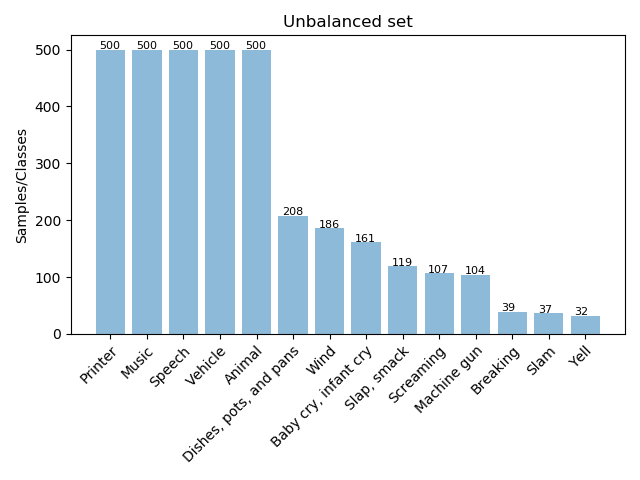
\includegraphics[scale=0.6]{samples-class-experiments}
		\caption{Bar plot that shows the number of samples for each of the selected classes. Clearly, the violent categories are much less populated than the others, that did not have to much any semantic criteria}
		\label{fig:mesh14}
	\end{figure}

	Some initial preprocessing were performed before passing the data to the different models. As mentioned in \ref{subsection:extracting-embeddings}, we had to deal with the zero-filling problem, which means that some of the rows of the embeddings matrices are completely zero because of the duration of the original video is less than 10s. As a solution, we decided to substitute the zero numbers in all the data with the machine epsilon\footnote{The machine epsilon value is considered the smallest value that satisfies $1 + \epsilon_{match} > 1$. It consists on the difference between one and the next closest number that is representable as a machine value \cite{Kaw}} value. 
	
	However, in the two models that use \acrshort{svm} for the multiclass classification a different solution was proposed. As it was explained in subsection \ref{label:svm}, this algorithm needs the input data matrix to be in the form [$number\ of\ samples\ \times\ number\ of\ features$], which differs from the originally shape of our data, [$number\ of\ samples\ \times\ number\ of\ seconds\ \times\ number\ of\ features$]. For this reason, we decided to reshape our data to the required form which resulted in a matrix of shape [$(number\ of\ samples\ \times\ number\ of\ seconds)\ \times\ number\ of\ features$]. With this conversion, instead of classifying full audio instances, the samples became the seconds of those instances. In order to remove zero data, we first checked the amount of zero-rows in every class. Since it was not very meaningful, we took them out of the dataset. 
	
	Once we had our data with all non-zero values, we needed to convert the set to balanced. First, for the classification task, we divided our data in train, validation and test subsets, using a 20\% for last one. Then, we decided to take out of the set half of the samples from the most populated classes \footnote{\textit{Speech}, \textit{Music}, \textit{Vehicle} and \textit{Animal}} from the train and validation sets, and generate new data for those with less observations by applying the data augmentation technique explained in subsection \ref{subsection:smote}. \doubt{This technique deduces a distribution for the given observations and generate synthetic samples within the distribution of each class until even the most populated category}. Just the train and validation set were subjected to this conversion, leaving the test set with the original embeddings. In figure \ref{fig:mesh15}, the subfigure (a) shows the distribution of data per class in the dataset for the case of the models that use \acrshort{svm} multiclass classifier. In subfigure (b), it is shown the distribution for the other four cases.
	
	\begin{figure}[ht]
		% Whole figure
		\captionsetup{justification=centering}
		\begin{subfigure}[b]{\textwidth}
			% Start with figure wav
			\centering
			\captionsetup{justification=centering}
			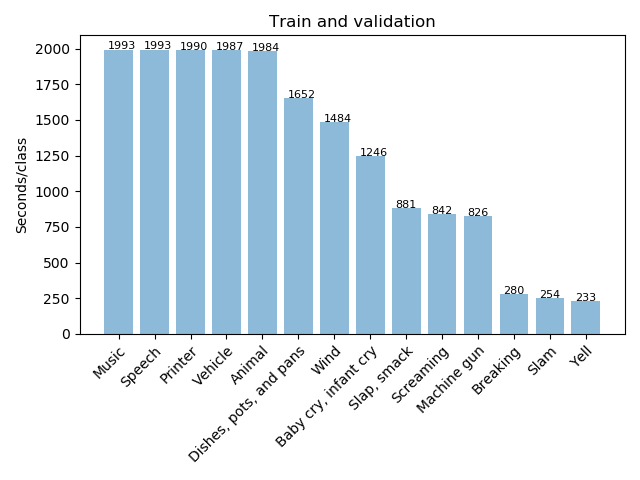
\includegraphics[width=0.5\linewidth]{tr_val_unbal_svm}%
			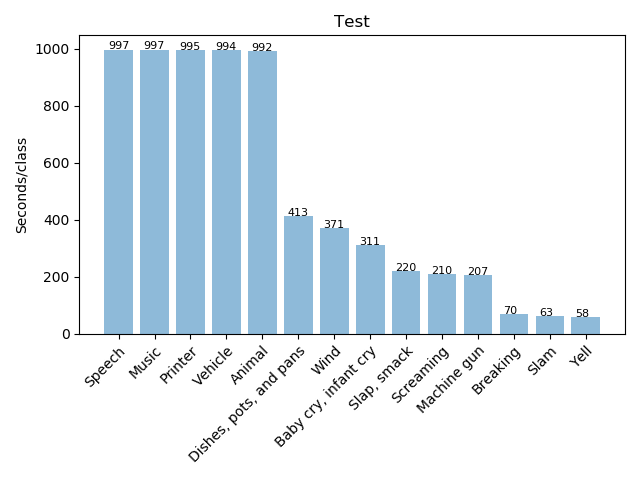
\includegraphics[width=0.5\linewidth]{tst_unbal_svm}
			\subcaption{This is the resulting subsets after downsampling the most populated classes and removing the zero-rows for the experiments that involve a SVM classifier}
		\end{subfigure}
		\vskip\baselineskip
		% Start with figure tfrecord
		\begin{subfigure}[b]{\textwidth}
			\centering
			\captionsetup{justification=centering}
			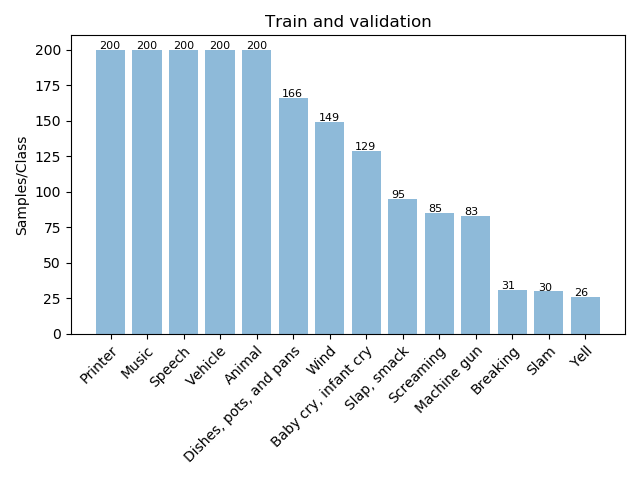
\includegraphics[width=0.5\linewidth]{tr_val_unbal}%
			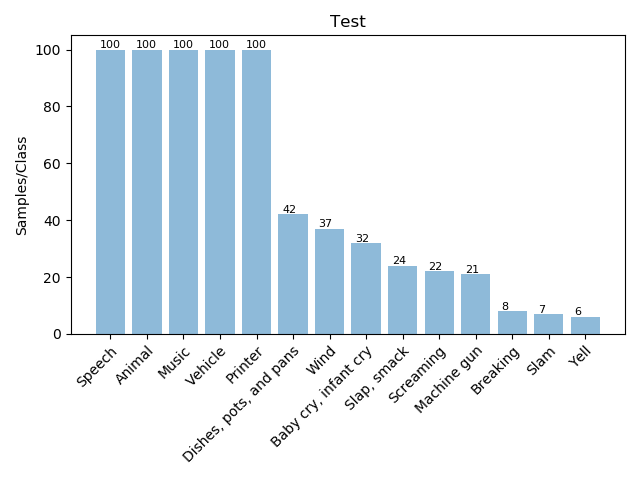
\includegraphics[width=0.5\linewidth]{tst_unbal}
			\subcaption{This is the resulting sets after downsampling the train and validation sets. The test set remains the same after the split}
		\end{subfigure}
		
		\caption{Number of observations for train, validation and test subsets used in the different experiments}
		\label{fig:mesh15}
	\end{figure}
	
	After these sets are obtained, the data augmentation technique \acrshort{smote} is applied. Finally, the shape input data for each of the experiments is shown in table \ref{table:8}
	
	\begin{table}[ht]
		\centering
		\begin{tabular}{|| m{7em} | m{10em} | m{10em} | m{10em} ||}
			\hline
			& \textbf{SVM multi and \acrshort{svm} + \acrshort{svm} binary} & \textbf{\acrshort{lstm} multi and \acrshort{lstm} + \acrshort{svm} binary} & \textbf{\acrshort{cnn} multi and \acrshort{cnn} + \acrshort{svm} binary}  \\
			\hline\hline
			\textbf{Train and validation} & 17645 (1993 per class) & 2800 (200 per class) & 2800 (200 per class) \\
			\hline
			\textbf{Test} & 6898 & 699 & 699 \\
			\hline                    
		\end{tabular}
		\caption{Train, validation and test set for different experiments}
		\label{table:8}
	\end{table}

\section{Implementations and results}

	For all the experiments, as mentioned above, the dataset was split by selecting a 20\% of the data for the testing procedure. The other part was divided into train and validation subsets with a \acrlong{kfold} technique, with 10 folds, which can also be called 10-fold cross-validation. A more detailed explanation about this resampling technique can be found in appendix \ref{appendix:kfold}. The average and standard deviation of the results for the different folds were obtained for training and validation. Then, a final measurement was performed for the test set. The way of checking the model performance was by finding the accuracy and confusion matrix, whose explanation can be found in appendix \ref{appendix:metrics}. For the cross-validation procedure, a matrix with the average values\footnote{In the average matrices, the results for each cell are shown just with one decimal in order to make a better and more comfortable visualization. However, the colour bar on the right of the plots must be taking into account since there might be some cells in which the value is $0.0$ but it is actually greater.} was obtained and also one for the standard deviation\footnote{In the standard deviation matrices the results are shown multiplied by $10^{2}$ in order to see the value in the different cells of the matrix} so the estimation of the model is represented for the corresponding subsets.
	
\subsection{Implementation 1: \acrshort{svm} classifier for a multiclass classification}

	Our first experiment consists of a \acrshort{svm} classifier that is used for a multiclass classification. In this case, we wanted to check the results of the performance of one of the most employed techniques in this filed different from \acrshort{nn}. It is true that this method is originally designed for binary problems but, as explained in \ref{subsection:svm}, we took advantage fo the multiclass algorithm. To define our model, we used mainly the default parameters. These includes of using a \acrshort{rbf} as a kernel. In this work, we have not investigated which type kernel could better fit our problem, however we found in the literature that the default option of \acrshort{rbf} is the most appropriated for real world applications \cite{Prajapati2010}. 
	
	In figure \ref{fig:mesh17}, a block diagram representation of the whole model is included. For this algorithm, the predicting labels \textit{\^{Y}}, are hard values, i.e. they correspond directly to the estimated label. 
	
	\begin{figure}[t]
		\centering
		\captionsetup{justification=centering}
		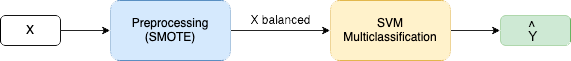
\includegraphics[scale=0.7]{svm-multi-block-diagram}
		\caption{SVM multiclass classifier whole model. \textit{X} is the input data that can be from train, validation or test set. \textit{\^{Y}} is the predicting labels for \textit{X}.}
		\label{fig:mesh17}
	\end{figure}

	Below, we can find the results for the different sets. In figure \ref{fig:mesh18}, the confusion matrices for the train and validation sets are shown. In figure \ref{fig:mesh19}, the confusion matrix for the evaluation on the test set is included. Finally, in the bar plot of figure \ref{fig:mesh20}, the accuracy values for the three sets are represented. For this case, the standard deviation is not shown for train and validation because it is zero when considering two decimals.
	
	\begin{figure}[ht]
		% Whole figure
		\captionsetup{justification=centering}
		\begin{subfigure}[b]{\textwidth}
			% Start with figure wav
			\captionsetup{justification=centering}
			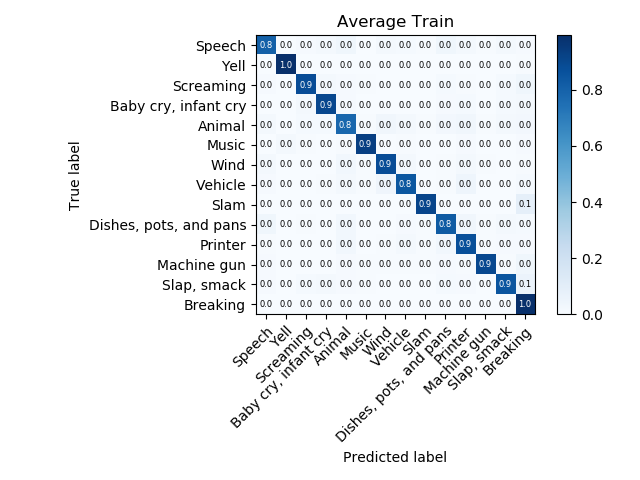
\includegraphics[width=0.6\linewidth]{svm-multi-cm-tr-av}%
			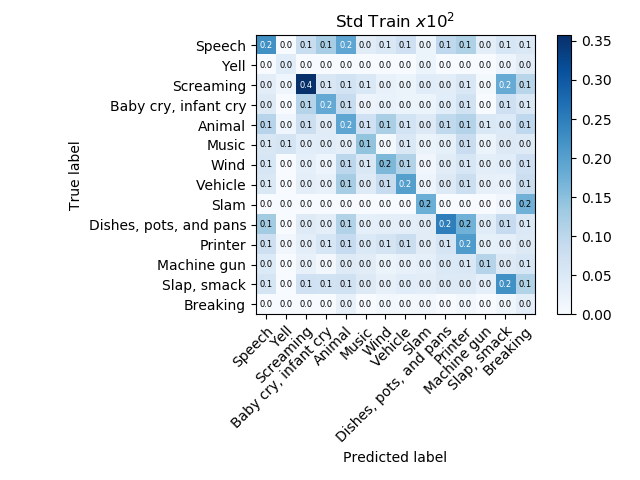
\includegraphics[width=0.6\linewidth]{svm-multi-cm-tr-std}
			\subcaption{Average and standard deviation for the train set}
		\end{subfigure}
		\vskip\baselineskip
		% Start with figure tfrecord
		\begin{subfigure}[b]{\textwidth}
			\captionsetup{justification=centering}
			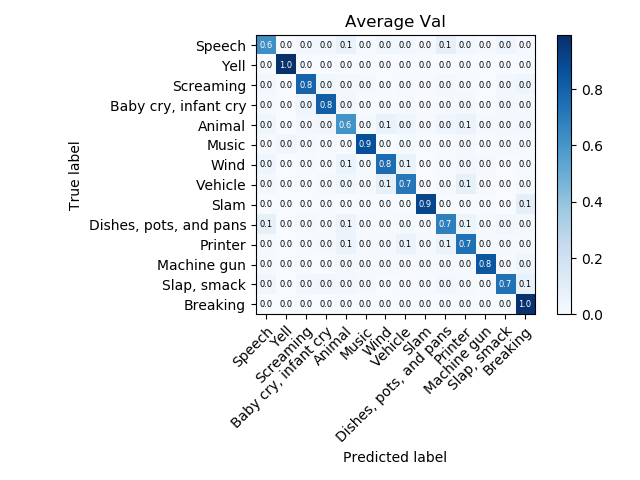
\includegraphics[width=0.6\linewidth]{svm-multi-cm-val-av}%
			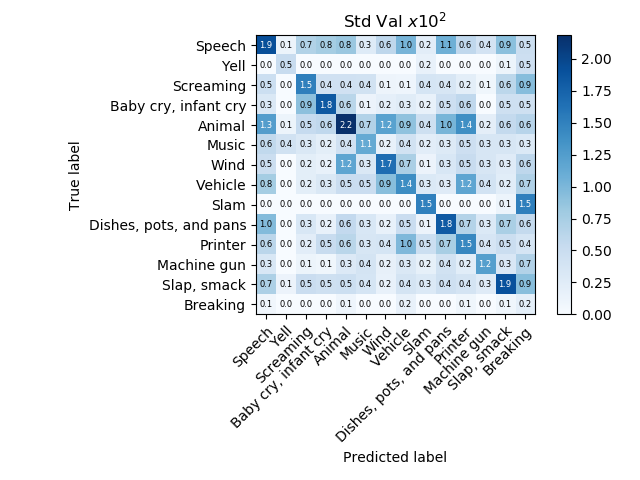
\includegraphics[width=0.6\linewidth]{svm-multi-cm-val-std}
			\subcaption{Average and standard deviation for the validation set}
		\end{subfigure}
		
		\caption{Confusion matrices for SVM multiclass classification for train and validation sets}
		\label{fig:mesh18}
	\end{figure}

	\begin{figure}[t]
		\centering
		\captionsetup{justification=centering}
		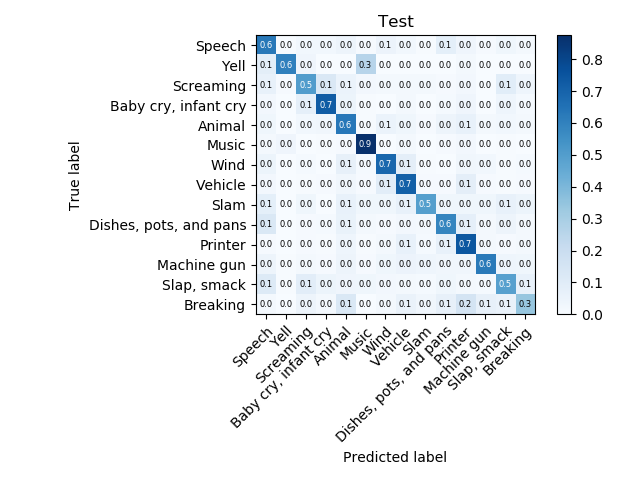
\includegraphics[width=0.8\linewidth]{svm-multi-cm-tst}
		\caption{Confusion matrix for the test set for the SVM multiclass classification}
		\label{fig:mesh19}
	\end{figure}

	\begin{figure}[t]
		\centering
		\captionsetup{justification=centering}
		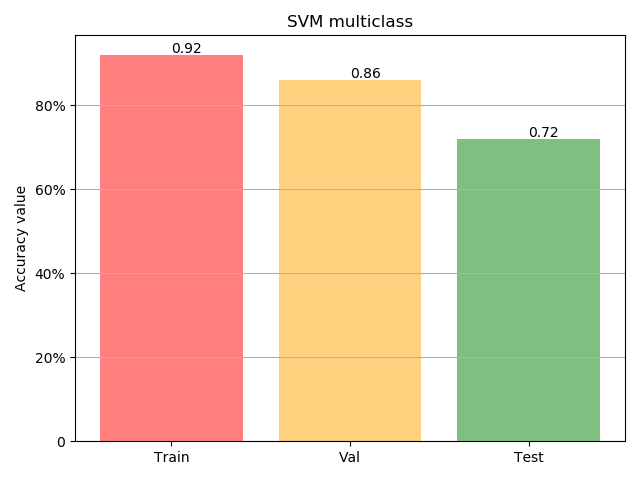
\includegraphics[width=0.8\linewidth]{svm-multierrorbar}
		\caption{Accuracy values for the three sets for the SVM multiclass classification}
		\label{fig:mesh20}
	\end{figure}

	
		
	
	
	
	
	
	
	
	
	
	
	